
Una \textit{template} \citep{okeeffe20261116densekuramotonetworks} \(T_m=(x,\phi, P)\) es una tripla tal que: 

\begin{itemize}
    \item \(x\): Las proporciones de los clústeres. \(x_a > 0\) y \(\sum^m x_a = 1\).
    \item \(\varphi\): Las fases de los clústeres.
    \item \(P\): La matriz de densidades interclúster. Es simétrica, y \(P_{ab}\) representa la fracción de uniones posibles entre dos clústeres. \(P_{ab} \in [0,1]\).
\end{itemize}

Algo útil, es que dados \((x,\phi)\) maximizar la conectividad es un problema semi-definido positivo y convexo, y \(\mu(T)=\min_a\sum_bP_{ab}x_b.\) \citep{okeeffe20261116densekuramotonetworks}. Por lo que convierte el problema de explorar grafos a explorar el espacio \((x,\phi)\).

Consideremos el estado de 4 clústeres  [Fig.~\ref{fig:c4}], que consta de cuatro grupos equidistribuidos con fases \(\varphi = (0, \pi/2, \pi, 3\pi/2)\).

\begin{figure}[htbp]
    \centering
    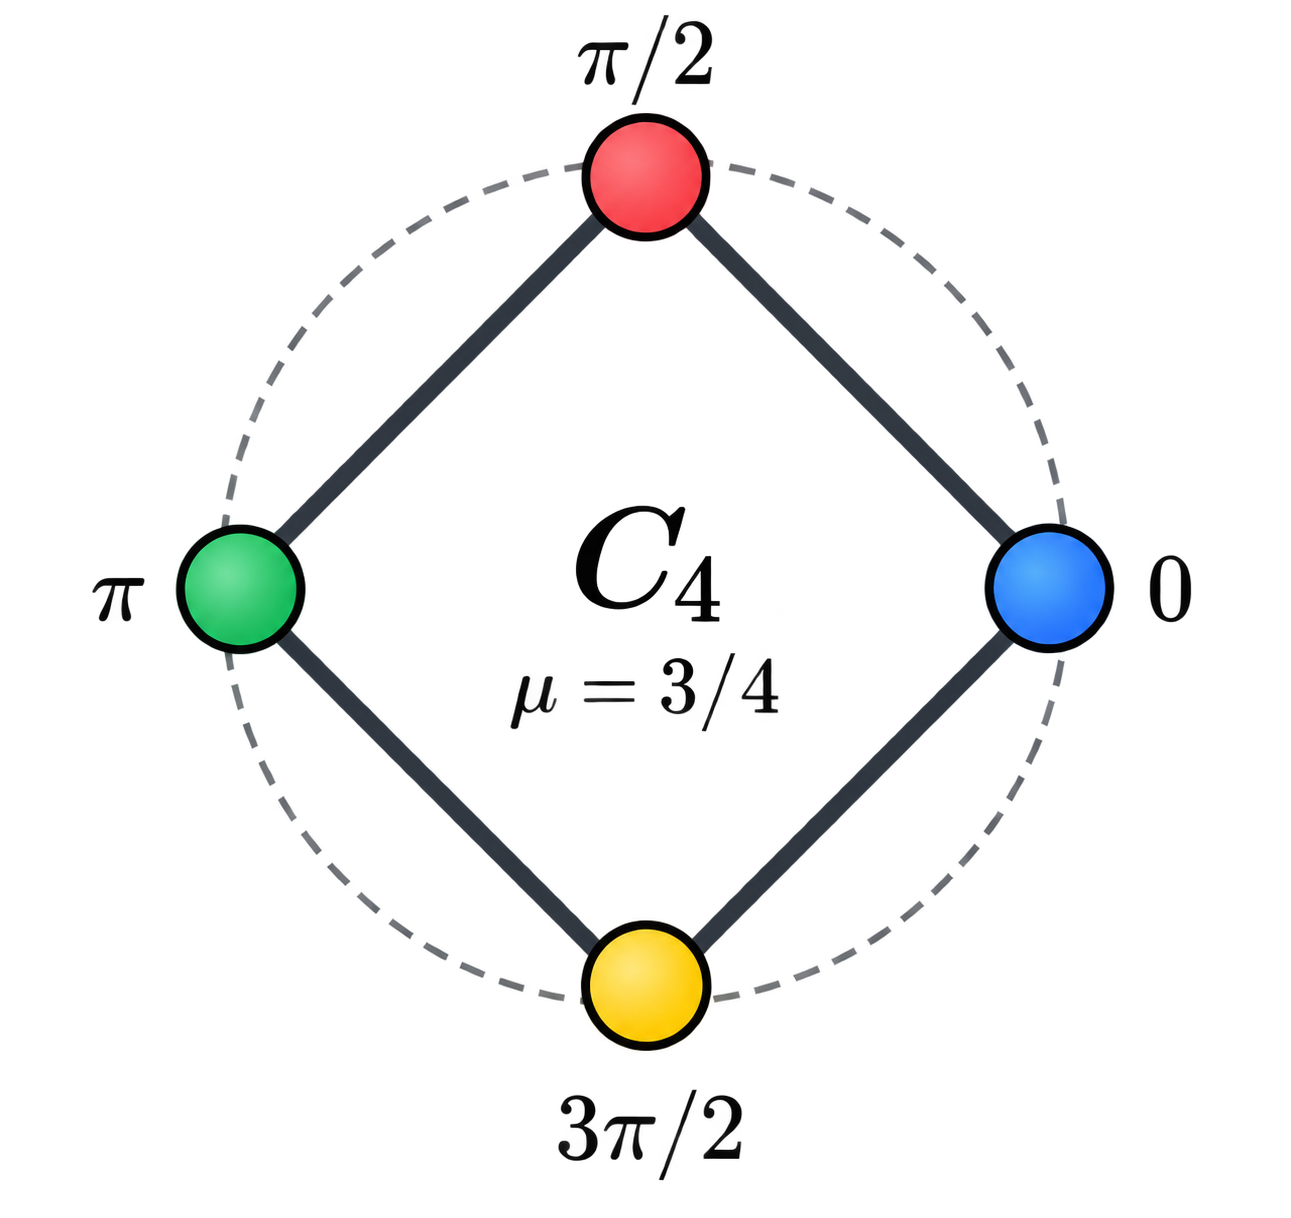
\includegraphics[width=\linewidth/4]{assets/C4.png}
    \caption{Estado \(C_4\).}
    \label{fig:c4}
\end{figure}

Se tiene que $\mu(C_4)=3/4$, pero este estado
no es estable. Kassabov, Strogatz y Townsend
\citep{Kassabov_2021} estudiaron este
estado degenerado, cuya estabilidad no puede
determinarse únicamente mediante el análisis lineal.
Además, $q(C_4)=1$.

Consideremos una conexion interclúster separados en fase en \(\pi/2\). Si perturbamos su fase por \(\epsilon\):

\[
sin(\frac{\pi}{2} + \epsilon) = cos(\epsilon) = 1 - \frac{\epsilon^2}{2} + O(\epsilon^4). 
\]

Por lo que a primer orden, el empuje recibido luego de una perturbación es proporcional a \(cos(\Delta\varphi)\), pero como \(\Delta\varphi = \pi/2\), sera 0.


El hessiano a nivel de clústeres tiene forma

\begin{equation}
    \mathcal{L}(y) = \sum_{a<b}{x_ax_bP_{ab}cos(\varphi_b-\varphi_a)(y_a-y_b)^2}
\end{equation}

En \(C_4\), cada conexión intergrupo tiene coseno 0 y, como grupos opuestos no están conectados directamente, obtenemos \(\mathcal{L}_{C_4}(y)=0\).

\subsection{Perturbaciones de \(C_4\)}

Consideremos
\begin{equation}
    \varphi_a(h) = \frac{\pi}{2}j(a) + hs_a
\end{equation}

Donde \(j(a)\in\{0,1,2,3\}\) identifica el grupo padre, \(s_a\) representa la desviación relativa del clúster \(a\) y \(h>0\) controla la magnitud de la perturbación. En este análisis mantenemos fijas las masas y excluimos
conexiones entre grupos padres opuestos:
\(P_{ab}(h)=0\) si \(j(b)-j(a)\equiv2\pmod4\).
Orientamos los enlaces vecinos de \(V_j\) hacia \(V_{j+1}\),
con índices módulo cuatro.

Por ejemplo, \(S_7\), el testigo de la mejor cota inferior obtenida por \cite{okeeffe20261116densekuramotonetworks}, se puede describir usando nuestra notación con 7 clústers \((-h,h,\pi/2-wh,\pi/2+wh, \pi-h, \pi+h, 3\pi/2)\).

En general, si \(\Delta_{ab} = s_b - s_a\), tenemos una diferencia de fases de \(\pi/2 + h\Delta_{ab}\) obteniendo un \textit{stiffness} de:

\[
\cos(\pi/2+h\Delta_{ab})
=-h\Delta_{ab}+O(h^3).
\]

\subsection{Condiciones de equilibrio}

Buscamos densidades de conexión que hagan estable
la perturbación. Para ello, expandimos
\begin{equation}
    P(h)=P^{(0)}+hP^{(1)}+O(h^2).
\end{equation}

La condición de equilibrio para cada clúster es
\begin{equation}
    F_a(h)=\sum_b x_bP_{ab}(h)
    \sin(\varphi_b(h)-\varphi_a(h))=0,
\end{equation}

Al expandir en potencias de $h$, exigimos
$F_a^{(0)}=F_a^{(1)}=0$.

Sea $V_j$ el conjunto de subclústeres del grupo
padre $j$, con índices módulo cuatro.
A orden cero obtenemos
\begin{equation}
    \sum_{b\in V_{j+1}}x_bP_{ab}^{(0)}
    =
    \sum_{b\in V_{j-1}}x_bP_{ab}^{(0)},
    \qquad a\in V_j.
    \label{eq:equilibrio_cero}
\end{equation}

A primer orden, las fuerzas internas deben ser
compensadas mediante cambios en las densidades:
\begin{equation}
\begin{aligned}
0=F_a^{(1)}
={}&\sum_{b\in V_j}
x_bP_{ab}^{(0)}(s_b-s_a)\\
&+\sum_{b\in V_{j+1}}x_bP_{ab}^{(1)}\\
&-\sum_{b\in V_{j-1}}x_bP_{ab}^{(1)}.
\end{aligned}
\label{eq:equilibrio_uno}
\end{equation}

Ambas condiciones son lineales en las densidades: la primera equilibra las interacciones entre grupos vecinos y la segunda compensa las fuerzas introducidas por la perturbación.

\subsection{Estabilidad a primer orden}

Consideremos perturbaciones colectivas $\eta_j$,
en las que todos los subclústeres del grupo
padre $j$ se desplazan conjuntamente.

Definimos
\begin{equation}
    K_j=
    \sum_{\substack{a\in V_j\\b\in V_{j+1}}}
    x_ax_bP_{ab}^{(0)}(s_b-s_a).
\end{equation}

La expansión del hessiano sobre estos movimientos es
\begin{equation}
    \mathcal{L}_h(\eta)
    =
    -h\sum_{j=0}^{3}
    K_j(\eta_j-\eta_{j+1})^2+O(h^2).
\end{equation}

Las condiciones de equilibrio a orden cero
implican que
\begin{equation}
    \sum_{j=0}^{3}K_j=0.
\end{equation}

Para que exista estabilidad, la matriz del término
de primer orden debe ser semidefinida positiva.
Pero esta matriz tiene traza
$-2\sum_j K_j=0$.

Una matriz semidefinida positiva de traza cero
debe ser nula. Por lo tanto,
\begin{equation}
    K_j=0 \qquad j=0,1,2,3.
    \label{eq:cancelacion_K}
\end{equation}

Es decir, la rigidez colectiva de primer orden
necesariamente se cancela. La estabilidad de los
modos colectivos debe aparecer a segundo orden.

\subsection{Estabilidad a segundo orden}

Para estudiar los modos débiles, consideramos
perturbaciones de la forma
\begin{equation}
    y_a=\eta_{j(a)}+hz_a,
\end{equation}
Para eliminar las redundancias entre movimientos
colectivos y relativos, imponemos
\[
    \sum_{a\in V_j}z_a=0
    \quad\forall j,
    \qquad
    \sum_j\eta_j=0.
\]
donde $\eta_j$ describe el movimiento colectivo
y $z_a$ el movimiento relativo de cada subclúster.

Definimos la energía interna
\begin{equation}
    I=
    \sum_j\sum_{\substack{a<b\\a,b\in V_j}}
    x_ax_bP_{ab}^{(0)}(s_a-s_b)^2.
\end{equation}
y los coeficientes
\begin{equation}
    k_j=
    -\sum_{\substack{a\in V_j\\b\in V_{j+1}}}
    x_ax_bP_{ab}^{(1)}(s_b-s_a).
\end{equation}

Las ecuaciones de equilibrio a primer orden
implican la identidad
\begin{equation}
    \sum_{j=0}^{3}k_j=I.
\end{equation}

La contribución de segundo orden al hessiano
se puede escribir como
\begin{equation}
    \mathcal{L}_h(\eta+hz)
    =
    h^2
    \begin{pmatrix}\eta\\z\end{pmatrix}^{T}
    \mathcal{H}_{\mathrm{lim}}
    \begin{pmatrix}\eta\\z\end{pmatrix}
    +O(h^3),
\end{equation}
donde
\begin{equation}
    \mathcal{H}_{\mathrm{lim}}=
    \begin{pmatrix}
        L_{\mathrm{cut}} & -G^T\\
        -G & L_{\mathrm{in}}
    \end{pmatrix}.
\end{equation}

Aquí $L_{\mathrm{cut}}$ describe la rigidez
entre grupos padres, $L_{\mathrm{in}}$ la rigidez
interna y $G$ el acoplamiento entre ambos tipos
de movimientos.

La condición necesaria de estabilidad es
\begin{equation}
    \mathcal{H}_{\mathrm{lim}}\succeq 0
    \label{eq:hessiano_limite}
\end{equation}
sobre los modos que excluyen la rotación global.

Cuando la rigidez interna es positiva en los
modos relativos, podemos minimizar respecto
de $z$ y obtener el complemento de Schur:
\begin{equation}
    Q_{\mathrm{eff}}
    =
    L_{\mathrm{cut}}
    -G^TL_{\mathrm{in}}^\dagger G.
\end{equation}

El término que se resta es semidefinido positivo:
permitir movimientos internos reduce la rigidez
efectiva de los grupos padres.

\subsection{Formulación mediante SDP}

\paragraph{Búsqueda externa.}
Partimos de cuatro grupos de masa $1/4$ asociados a $C_4$.
Exploramos los quince subconjuntos no vacíos de grupos que
pueden dividirse en dos masas iguales con desviaciones
opuestas, y añadimos divisiones desiguales independientes.
En una familia adicional impusimos las simetrías de $C_4$
que preservan cada partición. Optimizamos las masas y
desviaciones mediante SLSQP y refinamientos con
Nelder--Mead, resolviendo el SDP para cada geometría. Posteriormente exploramos particiones de hasta dieciséis
clústeres. El mejor resultado se obtuvo refinando en
aritmética exacta el patrón observado de tres pares y un
clúster único, seguido de una perturbación racional hacia
el interior de la región estable.

\paragraph{Optimizacion interna.}
Para masas, desviaciones y soporte fijos, las restricciones son lineales o semidefinidas y el problema es convexo. La búsqueda externa modifica la geometría y resuelve este SDP para cada candidato. Finalmente, las mejores soluciones se trasladan a \(h>0\). Los candidatos se validan inicialmente de forma
numérica. Para los mejores resultados se construyen
variantes racionales y se realizan las
certificaciones descritas posteriormente.
Durante la búsqueda fijamos un margen $\gamma>0$.
Denotamos por $\widehat{\mathcal H}_{\mathrm{lim}}$
la matriz de la forma límite en las coordenadas
reducidas anteriores.

\begin{equation}
\begin{aligned}
    \text{maximizar}\quad &\mu_0\\
    \text{sujeto a}\quad
        &F^{(0)}=0,\\
        &F^{(1)}=0,\\
        &K_j=0 \quad \forall j,\\
        &\sum_b x_bP_{ab}^{(0)}
            \geq\mu_0 \quad\forall a,\\
        &0\leq P_{ab}^{(0)}\leq1,\\
        &\hat{\mathcal{H}}_{\mathrm{lim}}\succeq \gamma I.
\end{aligned}
\label{eq:sdp_asintotico}
\end{equation}

Además, imponemos simetría de las matrices,
las restricciones del soporte, rigidez interna
positiva y correcciones $P^{(1)}$ admisibles
respecto de los límites de densidad.

\subsection{Resultados obtenidos}
La construcción $S_7$ de
\cite{okeeffe20261116densekuramotonetworks}
alcanza asintóticamente
\[
    \mu_{S_7}\approx 0.6929077063695864.
\]

Nosotros obtuvimos una familia
de templates estrictos que recuperan \(S_7\) desde perturbaciones de \(C_4\), con
\[
    \lim_{h\to0^+}\mu(T_h)=\mu_0,
    \qquad
    \boxed{\mu_0\ge 0.69290770636958636365.}
\]

\begin{figure}[htbp]
    \centering
    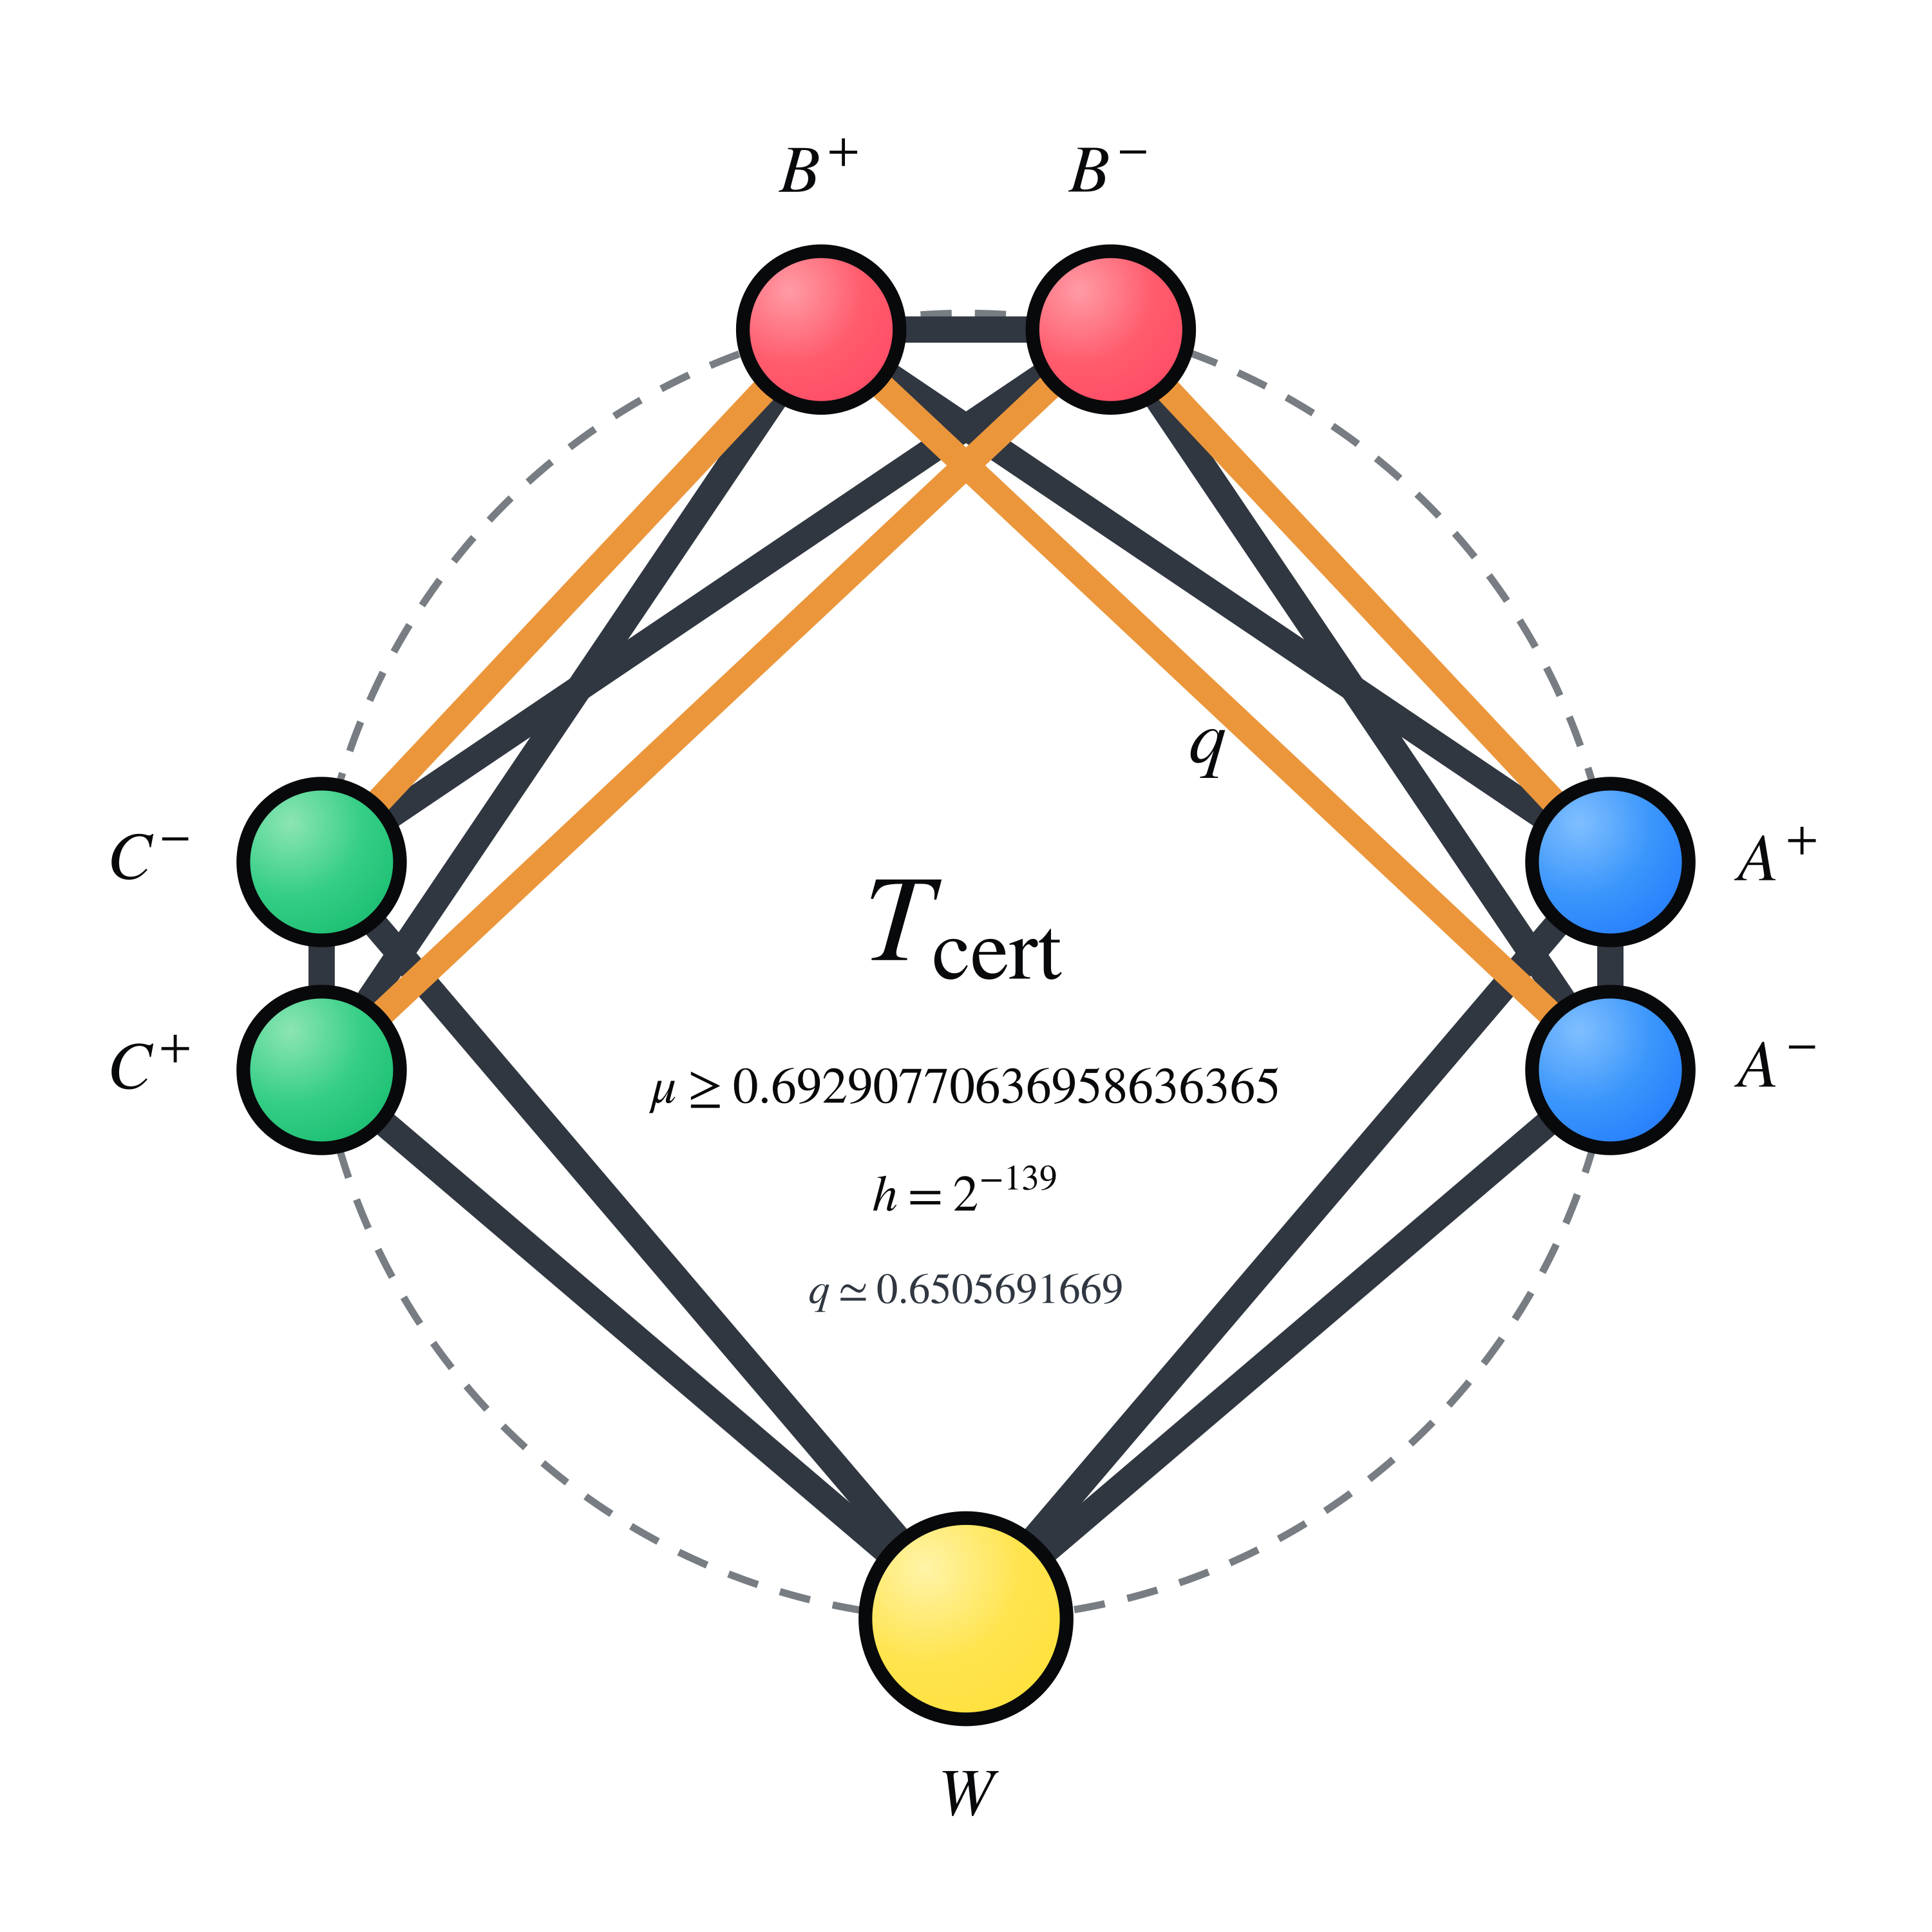
\includegraphics[width=0.3\linewidth]{assets/c4-certified-template-transparent.png}
    \caption{Template certificada, recupera \(S_7\).}
    \label{fig:template_cert}
\end{figure}

Para la familia asintótica se verificaron
exactamente las identidades de equilibrio y,
mediante Cholesky intervalar, la positividad del
hessiano límite; un argumento de levantamiento
establece la existencia para $h>0$ pequeño \citep{okeeffe20261116densekuramotonetworks}.
Para el template finito se verificaron el
equilibrio exacto, la inclusión de Krawczyk
y la estabilidad mediante Cholesky intervalar.

Las certificaciones corresponden a variantes
racionales próximas a las soluciones numéricas.
No superan la cota asintótica publicada ni
demuestran optimalidad global; tampoco se
proporciona una realización explícita en grafos
finitos.